\section{Preventivo}

La sezione Preventivo ha lo scopo di stimare il costo complessivo per la prestazione elargita. \\ 
La suddivisione oraria segue alcune regole comuni per ogni membro:
\begin{itemize}
	\item I componenti dovranno svolgere tutti i ruoli almeno una volta;
	\item Ogni componente dovrà lavorare almeno 8 ore per ogni ruolo;
	\item Tutti i componenti avranno lo stesso numero ore di lavoro ad ogni revisione.
\end{itemize}
Le sigle per i vari ruoli sono:
\begin{itemize}
	\item RE: Responsabile;
	\item AM: Amministratore;
	\item AN: Analista;
	\item PJ: Progettista;
	\item PR: Programmatore;
	\item VE: Verificatore.
\end{itemize}

\newpage
\subsection{Avvio ed Analisi dei Requisiti}
\subsubsection{Prospetto orario}

Nel periodo di \textit{Avvio ed Analisi dei Requisiti} la suddivisione oraria, per ogni membro del gruppo, è la seguente:

\begin{longtable}{|C{.30\textwidth}|C{.06\textwidth}|C{.06\textwidth}|C{.06\textwidth} | C{.06\textwidth}| C{.06\textwidth} | C{.06\textwidth} | C{.10\textwidth} |}
\hline
\textbf{Nome} & \textbf{RE} & \textbf{AM} & \textbf{AN} & \textbf{PJ} & \textbf{PR} & \textbf{VE} & \textbf{Totale}\\
\hline 
Marco Chilese & - & - & 10 & - & - & 15 & 25 \\
\hline
Marco Favaro & - & - & 14 & - & - & 11 & 25 \\
\hline
Diego Mazzalovo & - & - & 18 & - & - & 7 & 25 \\
\hline
Carlotta Segna & 11 & - & 5 & - & - & 9 & 25 \\
\hline
Matteo Slanzi & - & 8 & 10 & - & - & 7 & 25 \\
\hline
Bogdan Stanciu & 15 & - & 7 & - & - & 3 & 25\\
\hline
Luca Violato & - & 15 & 5 & - & - & 5 & 25 \\
\hline


\caption{Distribuzione oraria nel periodo di Avvio ed Analisi dei Requisiti}
\label{tab:dist oraria aar}
\end{longtable}

Il seguente grafico dà una visione grafica della suddivisione dei ruoli per il periodo di Avvio ed Analisi dei Requisiti:

\begin{figure}[H]
	\centering
  		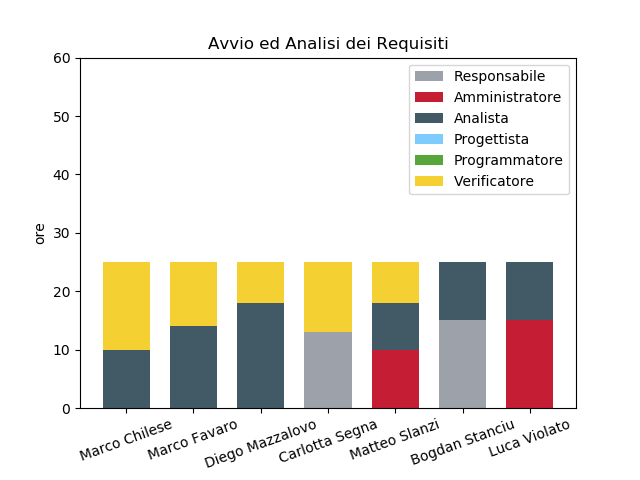
\includegraphics[width=1\linewidth]{./images/fig_aar.png}
  		\caption{Grafico suddivisione ore per persona nel periodo di Avvio ed Analisi dei Requisiti}
  		\label{fig:grafico suddivione ruoli aar}
\end{figure}



\subsubsection{Prospetto economico}
Nel periodo di \textit{Avvio ed Analisi dei Requisiti} la suddivisione oraria, per quanto riguarda i ruoli, è la seguente: 

\begin{longtable}{| C{.30\textwidth}| C{.15\textwidth}| C{.20\textwidth}|}
\hline
\textbf{Ruolo} & \textbf{Ore} & \textbf{Costo in \euro} \\
\hline
Responsabile & 26 & \EUR{780.00} \\
\hline
Amministratore & 23 & \EUR{460.00} \\
\hline
Analista & 69 & \EUR{1725.00} \\
\hline
Progettista & - & - \\
\hline
Programmatore & - & - \\
\hline
Verificatore & 57 & \EUR{855.00}\\
\hline
\textbf{Totale} & 175 & \EUR{3820.00} \\
\hline

\caption{Distribuzione oraria dei ruoli nel periodo di Avvio ed Analisi dei Requisiti}
\label{tab: distribuzione oraria aar}
\end{longtable}

Il seguente grafico dà una rappresentazione visiva della suddivisione dei ruoli:
\begin{figure}[H]
	\centering
  		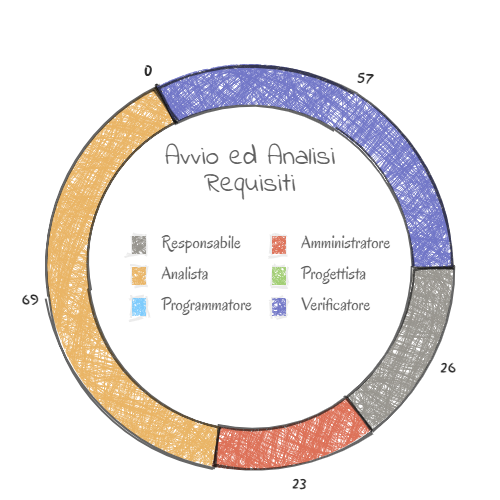
\includegraphics[width=0.8\linewidth]{./images/torta_aar.png}
  		\caption{Grafico suddivisione ruoli nel periodo di Avvio ed Analisi dei Requisiti}
  		\label{fig:grafico suddivione ruoli periodo di Avvio ed analisi dei requisiti}
\end{figure}

\subsection{Risanamento Criticità}
\subsubsection{Prospetto orario}

Nel periodo di \textit{Risanamento Criticità} la suddivisione oraria, per quanto riguarda i ruoli, è la seguente:

\begin{longtable}{|C{.30\textwidth}|C{.06\textwidth}|C{.06\textwidth}|C{.06\textwidth} | C{.06\textwidth}| C{.06\textwidth} | C{.06\textwidth} | C{.10\textwidth} |}
\hline
\textbf{Nome} & \textbf{RE} & \textbf{AM} & \textbf{AN} & \textbf{PJ} & \textbf{PR} & \textbf{VE} & \textbf{Totale}\\
\hline 
Marco Chilese & - & - & - & - & - & 7 & 7 \\
\hline
Marco Favaro & - & - & 7 & - & - & - & 7 \\
\hline
Diego Mazzalovo & - & - & 7 & - & - & - & 7 \\
\hline
Carlotta Segna & - & - & - & - & - & 7 & 7 \\
\hline
Matteo Slanzi & - & - & 7 & - & - & - & 7 \\
\hline
Bogdan Stanciu & 7 & - & - & - & - & - & 7 \\
\hline
Luca Violato & - & 7 & - & - & - & - & 7 \\
\hline

\caption{Distribuzione oraria nel periodo di Risanamento Criticità 1}
\label{Distribuzione oraria del periodo di rc1}
\end{longtable}



Il seguente grafico dà una visione grafica della suddivisione dei ruoli per il periodo di \textit{Risanamento criticità}:
\begin{figure}[H]
  \centering
  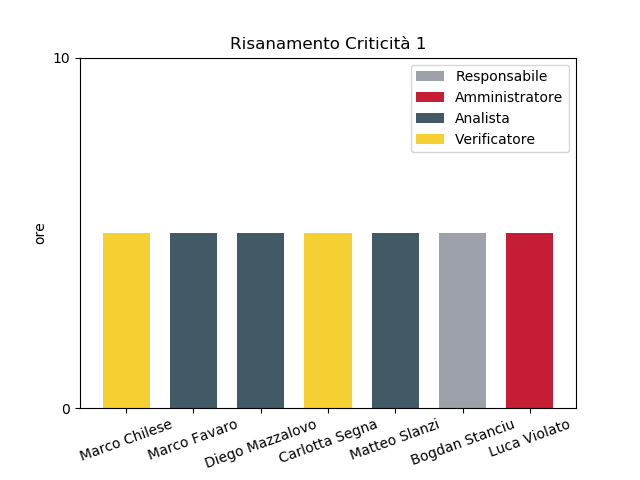
\includegraphics[width=1\linewidth]{./images/fig_rc1.png}
  \caption{Grafico suddivisione ore per persona nel periodo di Risanamento Criticità 1}
  \label{fig:grafico suddivione ruoli rc1}
\end{figure}

\subsubsection{Prospetto economico}
\begin{longtable}{| C{.30\textwidth}| C{.15\textwidth}| C{.20\textwidth}|}
\hline
\textbf{Ruolo} & \textbf{Ore} & \textbf{Costo in \euro} \\
\hline 
Responsabile & 7 & \EUR{210.00} \\
\hline
Amministratore & 7 & \EUR{140.00} \\
\hline
Analista & 21 & \EUR{525.00} \\
\hline
Progettista & - & - \\
\hline
Programmatore & - & - \\
\hline
Verificatore & 14 & \EUR{210.00}\\
\hline
\textbf{Totale} & 49 & \EUR{1085.00} \\
\hline


\caption{Distribuzione oraria dei ruoli nel periodo di Risanamento Criticità 1}
\label{Distribuzione oraria del periodo di rc1}
\end{longtable}

Il seguente grafico dà una rappresentazione visiva della suddivisione dei ruoli:
\begin{figure}[H]
	\centering
  		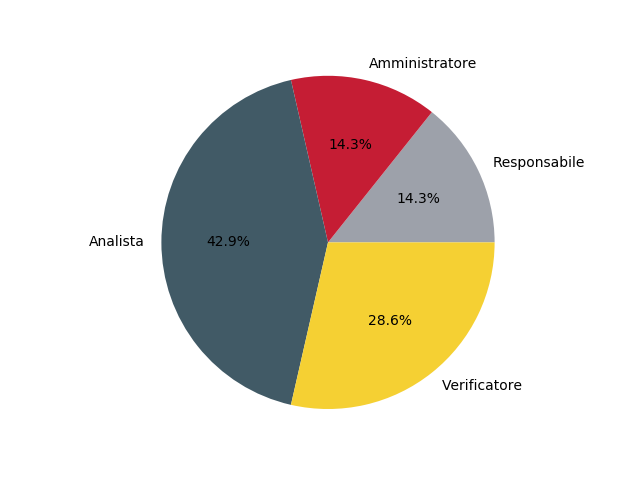
\includegraphics[width=0.8\linewidth]{./images/torta_rc1.png}
  		\caption{Grafico suddivisione ruoli nel periodo di Risanamento Criticità 1}
  		\label{fig:grafico suddivione ruoli periodo di rc1}
\end{figure}


\subsection{Progettazione Architetturale}
\subsubsection{Prospetto orario}

Nel periodo di \textit{Progettazione Architetturale} la suddivisione oraria, per ogni membro del gruppo, è la seguente:


\begin{longtable}{|C{.30\textwidth}|C{.06\textwidth}|C{.06\textwidth}|C{.06\textwidth} | C{.06\textwidth}| C{.06\textwidth} | C{.06\textwidth} | C{.10\textwidth} |}
\hline
\textbf{Nome} & \textbf{RE} & \textbf{AM} & \textbf{AN} & \textbf{PJ} & \textbf{PR} & \textbf{VE} & \textbf{Totale}\\
\hline 
Marco Chilese & - & 10 & - & 7 & 5 & - & 22 \\
\hline
Marco Favaro & 9 & - & 8 & - & - & 5 & 22 \\
\hline
Diego Mazzalovo & 8 & - & - & 7 & 7 & - & 22 \\ 
\hline
Carlotta Segna & - & - & 5 & 5 & 12 & - & 22 \\
\hline
Matteo Slanzi & - & - & 4 & - & 7 & 11 & 22 \\
\hline
Bogdan Stanciu & - & 8 & - & - & 14 & - & 22 \\
\hline
Luca Violato & - & - & 7 & 6 & - & 9 & 22 \\
\hline 

\caption{Distribuzione oraria del periodo di Progettazione Architetturale}
\label{Distribuzione oraria del periodo di pa}
\end{longtable}

Il seguente grafico dà una visione grafica della suddivisione dei ruoli per il periodo di Progettazione Architetturale:

\begin{figure}[H]
	\centering
  		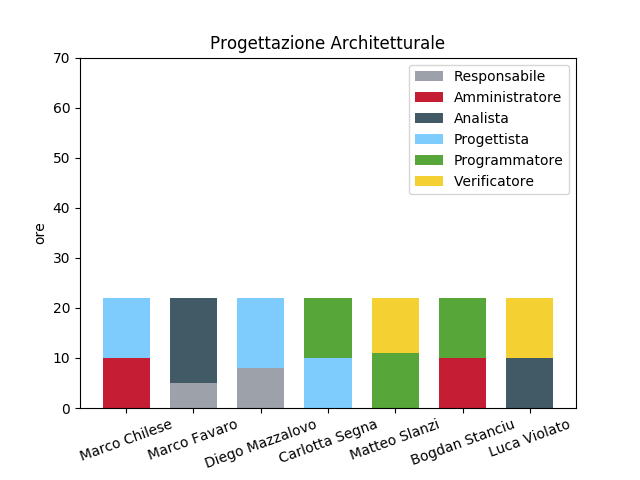
\includegraphics[width=1\linewidth]{./images/fig_pa.png}
  		\caption{Grafico suddivisione ore per persona nel periodo di Progettazione Architetturale}
  		\label{fig:grafico suddivione ruoli periodo di pa}
\end{figure}



\subsubsection{Prospetto economico}
\begin{longtable}{| C{.30\textwidth}| C{.15\textwidth}| C{.20\textwidth}|}
\hline
\textbf{Ruolo} & \textbf{Ore} & \textbf{Costo in \euro} \\
\hline 
Responsabile & 17 & \EUR{510.00} \\
\hline
Amministratore & 18 & \EUR{360.00}\\
\hline
Analista & 24 & \EUR{600.00} \\
\hline
Progettista & 25 & \EUR{550.00} \\
\hline
Programmatore & 45 & \EUR{675.00} \\
\hline
Verificatore & 25 & \EUR{375.00} \\
\hline
\textbf{Totale} & 154 & \EUR{3070.00}\\ 
\hline

\caption{Distribuzione oraria dei ruoli nel periodo di Progettazione Architetturale}
\label{Distribuzione oraria del periodo di pa}
\end{longtable}

Il seguente grafico dà una rappresentazione visiva della suddivisione dei ruoli:
\begin{figure}[H]
	\centering
  		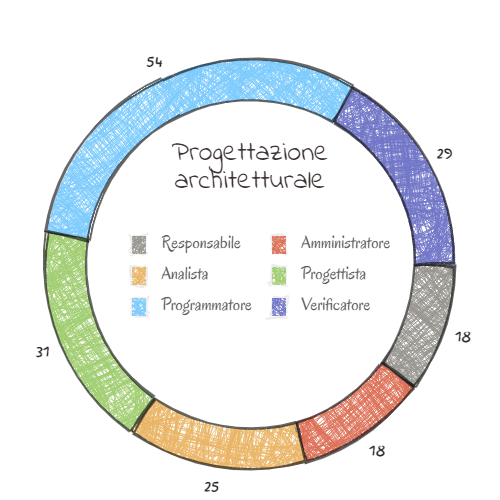
\includegraphics[width=0.8\linewidth]{./images/torta_pa.png}
  		\caption{Grafico suddivisione ruoli nel periodo di Progettazione Architetturale}
  		\label{fig:grafico suddivione ruoli pa}
\end{figure}


\subsection{Risanamento Criticità}
\subsubsection{Prospetto orario}

\begin{longtable}{|C{.30\textwidth}|C{.06\textwidth}|C{.06\textwidth}|C{.06\textwidth} | C{.06\textwidth}| C{.06\textwidth} | C{.06\textwidth} | C{.10\textwidth} |}
\hline
\textbf{Nome} & \textbf{RE} & \textbf{AM} & \textbf{AN} & \textbf{PJ} & \textbf{PR} & \textbf{VE} & \textbf{Totale}\\
\hline 
Marco Chilese & - & 5 & - & - & - & - & 5 \\
\hline
Marco Favaro & 5 & - & - & - & - & - & 5 \\
\hline
Diego Mazzalovo & - & - & - & 5 & - & - & 5 \\
\hline
Carlotta Segna & - & - & - & - & 5 & - & 5 \\
\hline
Matteo Slanzi & - & - & - & - & - & 5 & 5 \\
\hline
Bogdan Stanciu & - & - & 5 & - & - & - & 5 \\
\hline
Luca Violato & - & - & - & - & - & 5 & 5 \\   
\hline


\caption{Distribuzione oraria del periodo di Risanamento Criticità 2}
\label{Distribuzione oraria rc2}
\end{longtable}

Il seguente grafico dà una visione grafica della suddivisione dei ruoli per il periodo di \textit{Risanamento Criticità}:\begin{figure}[H]
	\centering
  		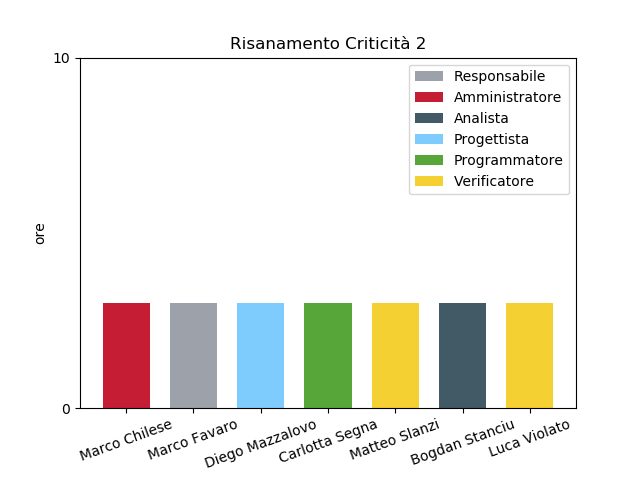
\includegraphics[width=1\linewidth]{./images/fig_rc2.png}
  		\caption{Grafico suddivisione ore per persona nel periodo di Risanamento Criticità 2}
  		\label{fig:grafico suddivione ruoli rc2}
\end{figure}



\subsubsection{Prospetto economico}
\begin{longtable}{| C{.30\textwidth}| C{.15\textwidth}| C{.20\textwidth}|}
\hline
\textbf{Ruolo} & \textbf{Ore} & \textbf{Costo in \euro} \\
\hline 
Responsabile & 5 & \EUR{150.00} \\
\hline
Amministratore & 5 & \EUR{100.00} \\
\hline
Analista & 5 & \EUR{125.00} \\
\hline
Progettista & 5 & \EUR{110.00}\\
\hline
Programmatore & 5 & \EUR{75.00} \\
\hline 
Verificatore & 10 & \EUR{150.00} \\
\hline
\textbf{Totale} & 35 & \EUR{710.00} \\
\hline 

\caption{Distribuzione oraria dei ruoli nel periodo di Risanamento Criticità 2}
\label{Distribuzione oraria rc2}
\end{longtable}

Il seguente grafico dà una rappresentazione visiva della suddivisione dei ruoli:
\begin{figure}[H]
	\centering
  		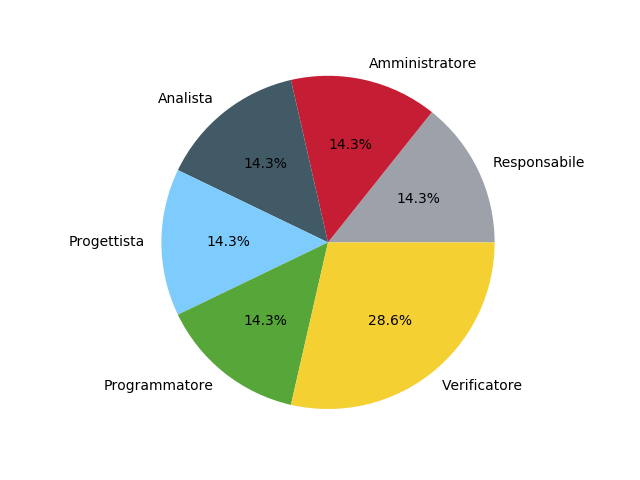
\includegraphics[width=0.8\linewidth]{./images/torta_rc2.png}
  		\caption{Grafico suddivisione ruoli nel periodo di Risanamento Criticità 2}
  		\label{fig:grafico suddivione ruoli rc2}
\end{figure}

\newpage
\subsection{Progettazione di Dettaglio e Codifica}
\subsubsection{Prospetto orario}

Nel periodo di \textit{Progettazione di Dettaglio e Codifica} la suddivisione oraria, per ogni membro del gruppo, è la seguente:

\begin{longtable}{|C{.30\textwidth}|C{.06\textwidth}|C{.06\textwidth}|C{.06\textwidth} | C{.06\textwidth}| C{.06\textwidth} | C{.06\textwidth} | C{.10\textwidth} |}
	\hline
	\textbf{Nome} & \textbf{RE} & \textbf{AM} & \textbf{AN} & \textbf{PJ} & \textbf{PR} & \textbf{VE} & \textbf{Totale}\\
	\hline 
	Marco Chilese & - & - & 8 & 16 & 16 & 10 & 50 \\
	\hline
	Marco Favaro &  - & - & - & 14 & 19 & 17 & 50 \\
	\hline
	Diego Mazzalovo & - & 8 & - & 11 & 20 & 11 & 50 \\
	\hline
	Carlotta Segna & - & 7 & - & 13 & 16 & 14 & 50 \\
	\hline
	Matteo Slanzi & 9 & - & 5 & 18 & 18 & - & 50 \\
	\hline
	Bogdan Stanciu & - & - & 10 & 22 & - & 18 & 50 \\
	\hline
	Luca Violato & 10 & - & - & 10 & 21 & 9 & 50 \\   
	\hline


\caption{Distribuzione oraria nel periodo di Progettazione di Dettaglio e Codifica}
\label{Distribuzione oraria pdc}
\end{longtable}

Il seguente grafico dà una visione grafica della suddivisione dei ruoli per il periodo di \textit{Progettazione di Dettaglio e Codifica}:

\begin{figure}[H]
	\centering
	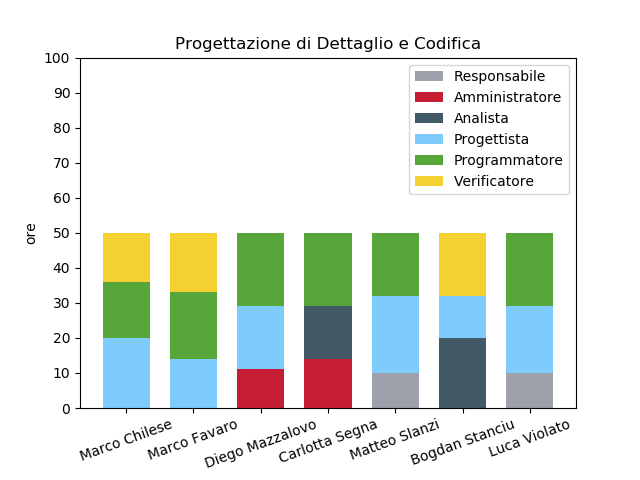
\includegraphics[width=1\linewidth]{./images/fig_pdc.png}
	\caption{Grafico suddivisione ore per persona nel periodo di Progettazione di Dettaglio e Codifica}
	\label{fig:grafico suddivione ruoli periodo pdc}
\end{figure}

\subsubsection{Prospetto economico}
\begin{longtable}{| C{.30\textwidth}| C{.15\textwidth}| C{.20\textwidth}|}
	\hline
	\textbf{Ruolo} & \textbf{Ore} & \textbf{Costo in \euro} \\
	\hline 
	Responsabile & 19 & \EUR{570.00} \\
	\hline
	Amministratore & 15 & \EUR{300.00}\\
	\hline
	Analista & 23 & \EUR{575.00} \\
	\hline
	Progettista & 104 & \EUR{2288.00} \\
	\hline
	Programmatore & 110 & \EUR{1650.00} \\
	\hline
	Verificatore & 79 & \EUR{1185.00} \\
	\hline
	\textbf{Totale} & 350 & \EUR{6568.00}\\ 
	\hline
	
	\caption{Distribuzione oraria del periodo di Progettazione di Dettaglio e Codifica}
	\label{Distribuzione oraria pdc}
\end{longtable}

Il seguente grafico dà una rappresentazione visiva della suddivisione dei ruoli:
\begin{figure}[H]
	\centering
	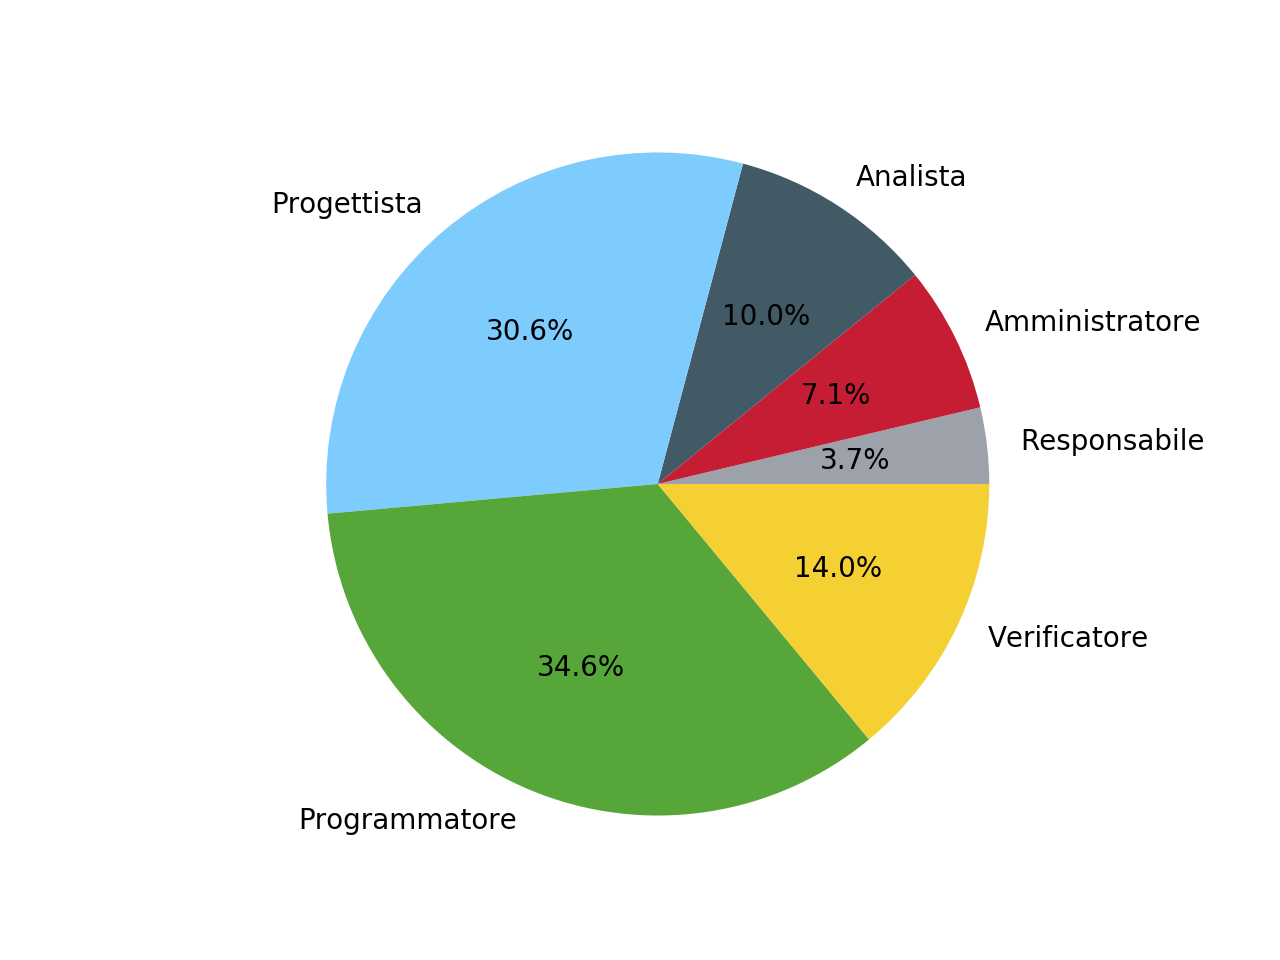
\includegraphics[width=0.8\linewidth]{./images/torta_pdc.png}
	\caption{Grafico suddivisione ore per persona nel periodo di Progettazione di Dettaglio e Codifica}
	\label{fig:grafico suddivione ruoli periodo pdc}
\end{figure}


\subsection{Risanamento Criticità}
\subsubsection{Prospetto orario}
\begin{longtable}{|C{.30\textwidth}|C{.06\textwidth}|C{.06\textwidth}|C{.06\textwidth} | C{.06\textwidth}| C{.06\textwidth} | C{.06\textwidth} | C{.10\textwidth} |}
	\hline
	\textbf{Nome} & \textbf{RE} & \textbf{AM} & \textbf{AN} & \textbf{PJ} & \textbf{PR} & \textbf{VE} & \textbf{Totale}\\
	\hline 
	Marco Chilese & - & - & 4 & - & - & - & 4 \\
	\hline
	Marco Favaro & - & - & - & - & - & 4 & 4 \\
	\hline
	Diego Mazzalovo & - & - & - & - & 4 & - & 4 \\
	\hline
	Carlotta Segna & - & 4 & - & - & - & - & 4 \\
	\hline
	Matteo Slanzi & - & - & - & - & 4 & - & 4 \\
	\hline
	Bogdan Stanciu & - & - & - & 4 & - & - & 4 \\
	\hline
	Luca Violato & 4 & - & - & - & - & - & 4 \\   
	\hline
	
	
	\caption{Distribuzione oraria del periodo di Risanamento Criticità 3}
	\label{Distribuzione oraria rc3}
\end{longtable}

Il seguente grafico dà una visione grafica della suddivisione dei ruoli per il periodo di Risanamento criticità:\begin{figure}[H]
	\centering
	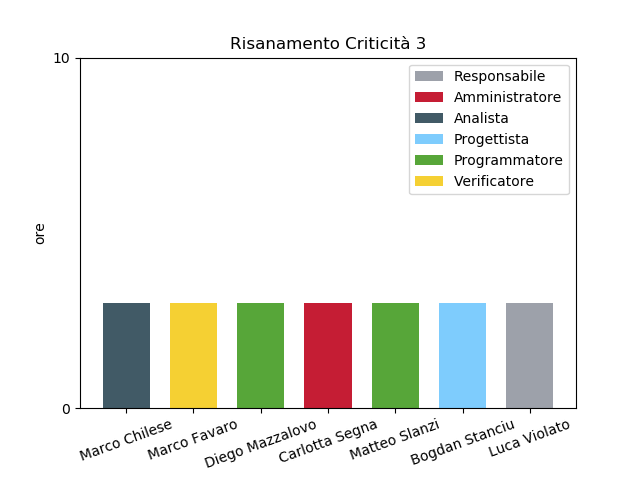
\includegraphics[width=1\linewidth]{./images/fig_rc3.png}
	\caption{Grafico suddivisione ore per persona nel periodo di Risanamento Criticità 3}
	\label{fig:grafico suddivione ruoli rc3}
\end{figure}

\subsubsection{Prospetto economico}
\begin{longtable}{| C{.30\textwidth}| C{.15\textwidth}| C{.20\textwidth}|}
	\hline
	\textbf{Ruolo} & \textbf{Ore} & \textbf{Costo in \euro} \\
	\hline 
	Responsabile & 4 & \EUR{120.00} \\
	\hline
	Amministratore & 4 & \EUR{80.00} \\
	\hline
	Analista & 4 & \EUR{100.00} \\
	\hline
	Progettista & 4 & \EUR{88.00}\\
	\hline
	Programmatore & 8 & \EUR{120.00} \\
	\hline 
	Verificatore & 4 & \EUR{60.00} \\
	\hline
	\textbf{Totale} & 28 & \EUR{568.00} \\
	\hline 


\caption{Distribuzione oraria dei ruoli nel periodo di Risanamento Criticità 3}
\label{Distribuzione oraria rc3}
\end{longtable}

Il seguente grafico dà una visione grafica della suddivisione dei ruoli per il periodo di Risanamento Criticità:\begin{figure}[H]
	\centering
	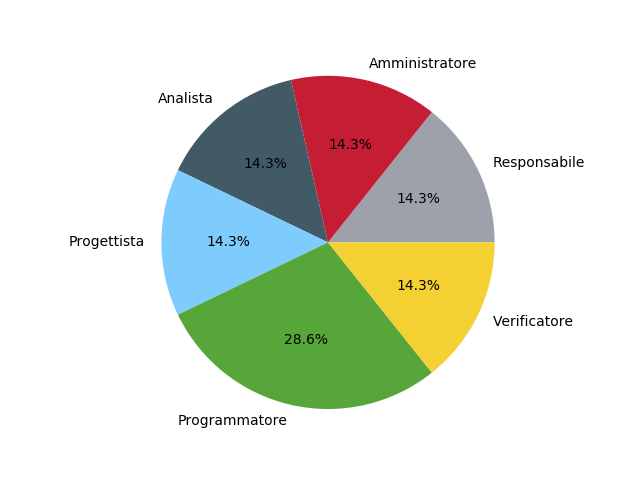
\includegraphics[width=0.8\linewidth]{./images/torta_rc3.png}
	\caption{Grafico suddivisione ruoli nel periodo di Risanamento Criticità 3}
	\label{fig:grafico suddivione ruoli rc3}
\end{figure}

\newpage

\subsection{Validazione e Collaudo}
\subsubsection{Prospetto orario}
Nel periodo di \textit{Validazione e Collaudo} la suddivisione oraria, per ogni membro del gruppo, è la seguente:

\begin{longtable}{|C{.30\textwidth}|C{.06\textwidth}|C{.06\textwidth}|C{.06\textwidth} | C{.06\textwidth}| C{.06\textwidth} | C{.06\textwidth} | C{.10\textwidth} |}
	\hline
	\textbf{Nome} & \textbf{RE} & \textbf{AM} & \textbf{AN} & \textbf{PJ} & \textbf{PR} & \textbf{VE} & \textbf{Totale}\\
	\hline 
	Marco Chilese & 8 & - & - & - & 5 & 9 & 22 \\
	\hline
	Marco Favaro &  - & 11 & - & - & 3 & 8 & 22 \\
	\hline
	Diego Mazzalovo & - & - & - & 6 & 6 & 10 & 22 \\
	\hline
	Carlotta Segna & - & 6 & - & 4 & 5 & 7 & 22 \\
	\hline
	Matteo Slanzi & - & - & - & 7 & 6 & 9 & 22 \\
	\hline
	Bogdan Stanciu & - & - & - & 5 & 8 & 9 & 22 \\
	\hline
	Luca Violato & - & - & - & - & 10 & 12 & 22 \\   
	\hline
	
	
	\caption{Distribuzione oraria nel periodo di Validazione e Collaudo}
	\label{Distribuzione oraria vc}
\end{longtable}

Il seguente grafico dà una visione grafica della suddivisione dei ruoli per il periodo di \textit{Validazione e Collaudo}:

\begin{figure}[H]
	\centering
	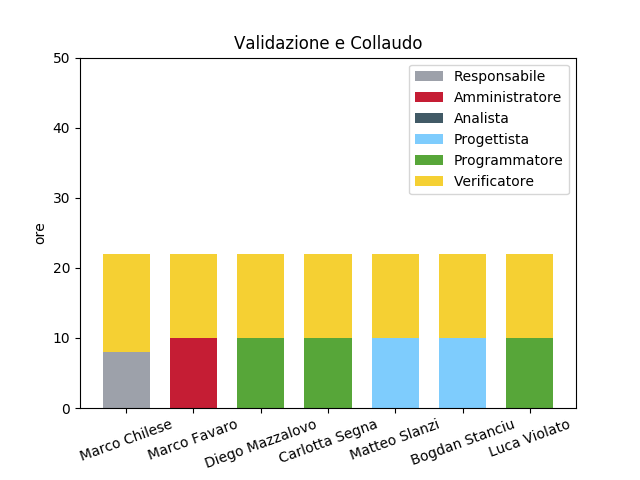
\includegraphics[width=1\linewidth]{./images/fig_vc.png}
	\caption{Grafico suddivisione ore per persona nel periodo di Validazione e Collaudo}
	\label{fig:grafico suddivione ruoli periodo vc}
\end{figure}

\begin{longtable}{| C{.30\textwidth}| C{.15\textwidth}| C{.20\textwidth}|}
	\hline
	\textbf{Ruolo} & \textbf{Ore} & \textbf{Costo in \euro} \\
	\hline 
	Responsabile & 8 & \EUR{240.00} \\
	\hline
	Amministratore & 17 & \EUR{340.00}\\
	\hline
	Analista & 0 & \EUR{0.00} \\
	\hline
	Progettista & 22 & \EUR{484.00} \\
	\hline
	Programmatore & 43 & \EUR{645.00} \\
	\hline
	Verificatore & 64 & \EUR{960.00} \\
	\hline
	\textbf{Totale} & 154 & \EUR{2669.00}\\ 
	\hline
	
	\caption{Distribuzione oraria dei ruoli nel periodo di Validazione e Collaudo}
	\label{Distribuzione oraria del periodo di Validazione e collaudo}
\end{longtable}

Il seguente grafico dà una rappresentazione visiva della suddivisione dei ruoli:
\begin{figure}[H]
	\centering
	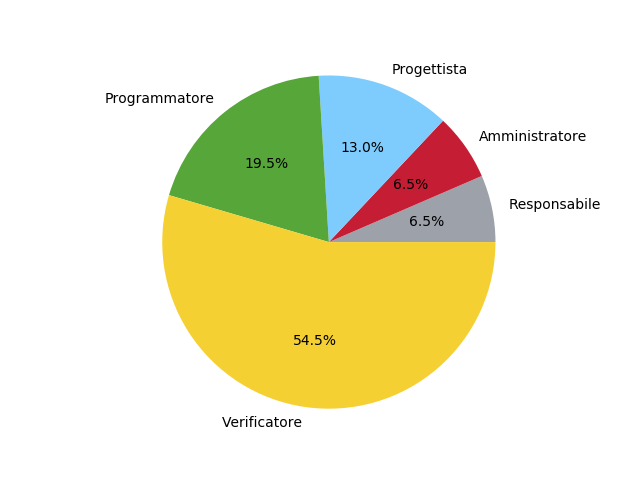
\includegraphics[width=0.8\linewidth]{./images/torta_vc.png}
	\caption{Grafico suddivisione ruoli nel periodo di Validazione e Collaudo}
	\label{fig:grafico suddivione ruoli periodo di Validazione e collaudo}
\end{figure}

\newpage

\subsection{Totale ore rendicontate}
\subsubsection{Prospetto orario}

Le ore di seguito riportate sono da considerarsi a carico del committente, che non includono le ore della prima fase:

\begin{longtable}{|C{.30\textwidth}|C{.06\textwidth}|C{.06\textwidth}|C{.06\textwidth} | C{.06\textwidth}| C{.06\textwidth} | C{.06\textwidth} | C{.10\textwidth} |}
\hline
\textbf{Nome} & \textbf{RE} & \textbf{AM} & \textbf{AN} & \textbf{PJ} & \textbf{PR} & \textbf{VE} & \textbf{Totale}\\
\hline 
Marco Chilese & 8 & 15 & 12 & 23 & 26 & 26 & 110\\
\hline
Marco Favaro & 14 & 11 & 15 & 14 & 22 & 34 & 110\\
\hline
Diego Mazzalovo & 8 & 8 & 7 & 29 & 37 & 21 & 110\\
\hline
Carlotta Segna & - & 17 & 5 & 22 & 38 & 28 & 110\\
\hline
Matteo Slanzi & 9 & - & 16 & 25 & 35 & 25 & 110\\
\hline
Bodgan Stanciu & 7 & 8 & 15 & 31 & 22 & 27 & 110\\
\hline
Luca Violato & 14 & 7 & 7 & 16 & 31 & 35 & 110 \\
\hline

\caption{Distribuzione oraria delle ore rendicontate}
\label{Distribuzione oraria delle ore rendicontate}
\end{longtable}

Il seguente grafico dà una visione grafica della suddivisione dei ruoli per il periodo di Risanamento criticità:%\begin{figure}[H]

\begin{figure}[H]
	\centering
  		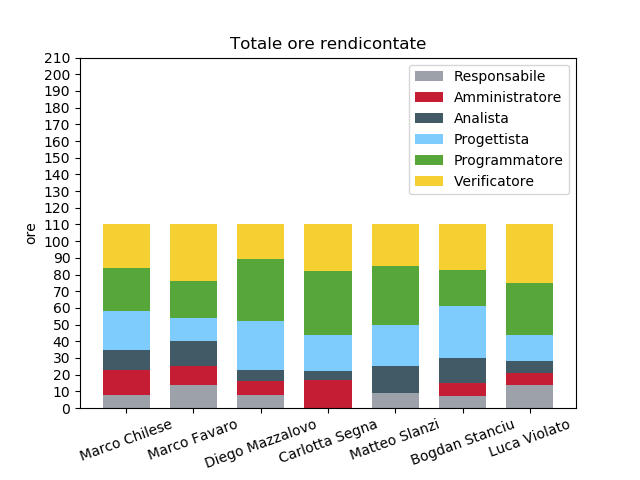
\includegraphics[width=1\linewidth]{./images/fig_tor.png}
  		\caption{Grafico suddivisione ruoli rendicontati}
  		\label{fig:grafico suddivione ruoli}
\end{figure}


\subsubsection{Prospetto economico}
\begin{longtable}{| C{.30\textwidth}| C{.15\textwidth}| C{.20\textwidth}|}
\hline
\textbf{Ruolo} & \textbf{Ore} & \textbf{Costo in \euro} \\
\hline
Responsabile & 60 & \EUR{1800.00} \\
\hline
Amministratore & 66 & \EUR{1320.00} \\
\hline
Analista & 77 & \EUR{1925.00} \\
\hline
Progettista & 160 & \EUR{3520.00}\\
\hline 
Programmatore & 211 & \EUR{3165.00} \\
\hline
Verificatore & 196 & \EUR{2940.00} \\
\hline 
\textbf{Totale} & 770 & \EUR{14670.00}\\
\hline

\caption{Distribuzione oraria dei ruoli delle ore rendicontate}
\label{Distribuzione oraria a carico del committente}
\end{longtable}

\begin{figure}[H]
	\centering
  		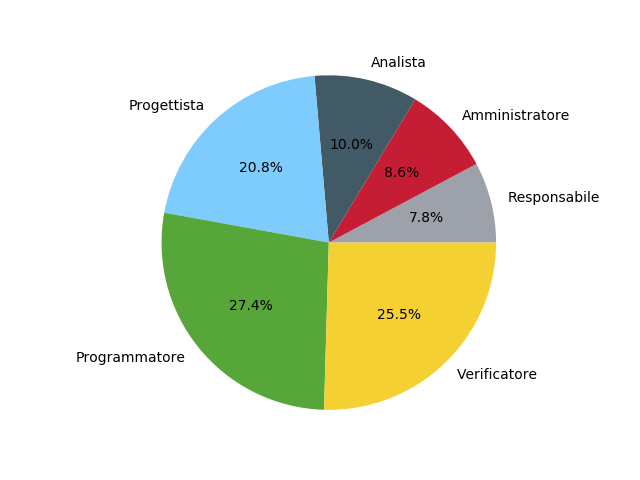
\includegraphics[width=0.8\linewidth]{./images/torta_to.png}
  		\caption{Grafico suddivisione ruoli rendicontati}
  		\label{fig:grafico suddivione ruoli}
\end{figure}



\subsection{Totale ore con investimento}
\subsubsection{Prospetto orario}


\begin{longtable}{|C{.30\textwidth}|C{.06\textwidth}|C{.06\textwidth}|C{.06\textwidth} | C{.06\textwidth}| C{.06\textwidth} | C{.06\textwidth} | C{.10\textwidth} |}
\hline
\textbf{Nome} & \textbf{RE} & \textbf{AM} & \textbf{AN} & \textbf{PJ} & \textbf{PR} & \textbf{VE} & \textbf{Totale}\\
\hline 
Marco Chilese & 8 & 15 & 22 & 23 & 26 & 41 & 135\\
\hline
Marco Favaro & 14 & 11 & 29 & 14 & 22 & 45 & 135\\
\hline
Diego Mazzalovo & 8 & 8 & 25 & 29 & 37 & 28 & 135\\
\hline
Carlotta Segna & 11 & 17 & 10 & 22 & 38 & 37 & 135\\
\hline
Matteo Slanzi & 9 & 8 & 26 & 25 & 35 & 32 & 135\\
\hline
Bodgan Stanciu & 22 & 8 & 22 & 31 & 22 & 30 & 135\\
\hline
Luca Violato & 14 & 22 & 12 & 16 & 31 & 40 & 135 \\
\hline


\caption{Distribuzione oraria con investimento}
\label{Distribuzione oraria delle ore con investimento}
\end{longtable}

\begin{figure}[H]
	\centering
  		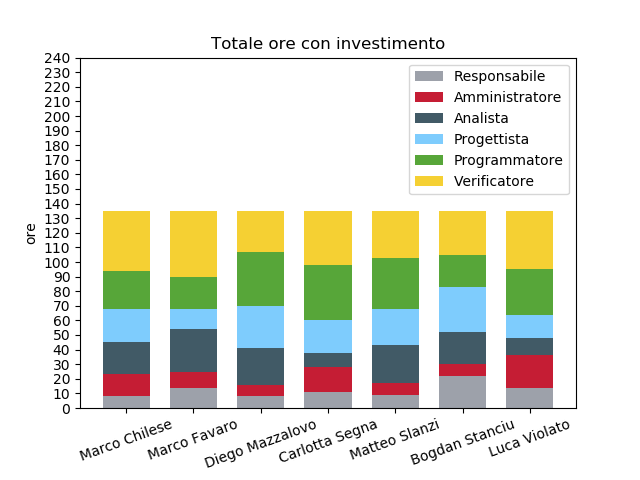
\includegraphics[width=1\linewidth]{./images/fig_toi.png}
  		\caption{Grafico suddivisione ruoli con investimento}
  		\label{fig:grafico suddivione ruoli con investimento}
\end{figure}

\subsubsection{Prospetto economico}

\begin{longtable}{| C{.30\textwidth}| C{.15\textwidth}| C{.20\textwidth}|}
\hline
\textbf{Ruolo} & \textbf{Ore} & \textbf{Costo in \euro} \\
\hline 
Responsabile & 86 & \EUR{2580.00}\\
\hline
Amministratore & 89 & \EUR{1780.00} \\
\hline
Analista & 146 & \EUR{3650.00} \\
\hline 
Progettista & 160 & \EUR{3520.00}\\
\hline
Programmatore & 211 & \EUR{3165.00} \\
\hline
Verificatore & 253 & \EUR{3795.00} \\
\hline
\textbf{Totale} & 945 & \EUR{18490.00} \\
\hline
\caption{Distribuzione oraria dei ruoli con investimento}
\label{Distribuzione oraria ruoli con investimento}
\end{longtable}

\begin{figure}[H]
	\centering
  		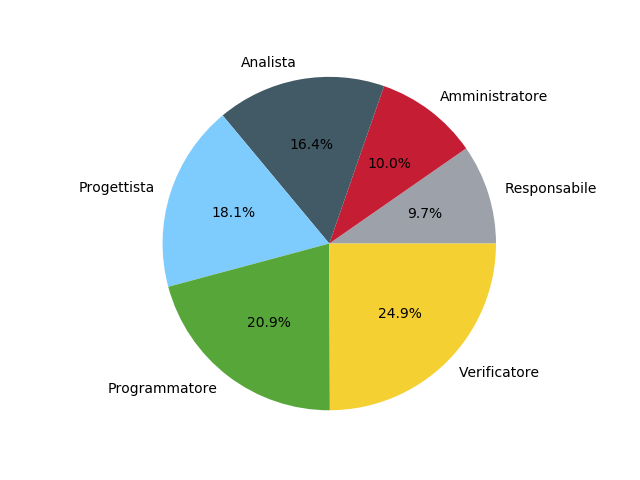
\includegraphics[width=0.8\linewidth]{./images/torta_toci.png}
  		\caption{Grafico suddivisione ruoli con investimento}
  		\label{fig:grafico suddivione ruoli con investimento}
\end{figure}



